% This file is iccc.tex.  It contains the formatting instructions for and acts as a template for submissions to ICCC.  It borrows liberally from the AAAI and IJCAI formats and instructions.  It uses the files iccc.sty, iccc.bst and iccc.bib, the first two of which also borrow liberally from the same sources.


\documentclass[letterpaper]{article}
\usepackage{iccc}
\usepackage{times}
\usepackage{helvet}
\usepackage{courier}
\usepackage{graphicx}
\usepackage{amsmath}
\usepackage{amssymb}

\graphicspath{ {images/} }

\newcommand\mydots{\hbox to .75em{.\hss.\hss.}}

\pdfinfo{
/Title (Human-Level Concept Learning in Computational Creativity)
/Subject (Proceedings of ICCC)
/Author (Paul Bodily)}
% The file iccc.sty is the style file for ICCC proceedings.
%
\title{Human-Level Concept Learning in Computational Creativity}
\author{Paul Bodily, Benjamin Bay, and Dan Ventura\\
Computer Science Department\\
Brigham Young University\\
Provo, UT 84602  USA\\
paulmbodily@gmail.com, benjamin.bay@gmail.com, ventura@cs.byu.edu\\
}
\setcounter{secnumdepth}{0}

\begin{document} 
\maketitle
\begin{abstract}
\begin{quote}
In Hierarchical Bayesian program learning (HBPL) trained models for subconcepts are combined to achieve human-like results in one-shot classification, parsing, and generation of hand-written characters. We contend that the HBPL framework is well-suited for modeling creative artefacts inasmuch as it allows explicit modeling of intention, structure, and substructure. We discuss issues related to factoring joint distributions over artefact classes generally, using lyrical composition as a specific example. How joint distributions are factored largely reflects the philosophical debates that occur among artists themselves, suggesting that the HBPL framework might serve as a more precise scaffolding for such debates. Besides generating, the concept-learning framework naturally lends itself to broader applications, including recommendation systems.
\end{quote}
\end{abstract}

\section{Introduction}

People possess the amazing ability to learn and combine concepts they already know to understand and even create new concepts. As an example, by many pedagogical models (e.g., \cite{englemann1974distar}) children learn to read by systematically mastering and combining simple concepts: symbols represent sounds; symbols are read left to right; sounds can be combined to form words (an already familiar concept); periods delimit phrases; sentences wrap to subsequent lines, etc. This process of hierarchical learning is at the heart of a branch of machine learning called \textit{human-level concept learning}. Human-level concept-learning is characterized by three fundamental ideas \cite{lake2015human}:

\begin{itemize}  
\item \emph{Compositionality} - observations are constructed through a combination of parts
\item \emph{Causality} - capturing abstract representations of the causal process that produces an artefact
\item \emph{Learning-to-learn} - parameters, constraints, parts, etc. are learned from training with related concepts and then applied to learning novel concepts
\end{itemize}

Hierarchical Bayesian program learning (HBPL) describes a framework that models human-level concept learning. This framework has recently been shown to be extremely effective (better even than deep-learning algorithms) in one-shot classification, parsing, and generation of hand-written characters \cite{lake2015human}. The HBPL model for hand-written characters works by factoring a joint probability distribution over characters into a product of conditional distributions,

\begin{equation} \label{eq:1}
P(\psi) = P(\kappa) \prod_{i=1}^{\kappa} P(n_i|\kappa)P(S_i|i,n_i)P(R_i|S_1, ..., S_{i-1}),
\end{equation}

\noindent where each conditional distribution is a model of a \textit{subconcept}: \( P(\kappa) \) models the number of strokes per character; \( P(n_i|\kappa) \) models the \# of substrokes for the $i$th stroke for a character with $\kappa$ strokes; \( P(S_i|i,n_i) \) models the $i$th stroke with $n_i$ substrokes; and \( P(R_i|S_1, ..., S_{i-1}) \) models the relation of the $i$th stroke to the previous strokes. Each of these models can be further decomposed. This process of decomposition allows the system to effectively learn subconcepts from empirical data in order to easily learn and generate new character types.

In this paper we investigate the strengths and weaknesses of human-level concept learning as a tool for creating computationally creative systems. In particular we find that the HBPL model provides a powerful framework for producing novel, typical, artefacts that invariably include elements of surprise by virtue of its wide range of expression.

As a proof of concept, we demonstrate the application of the HBPL model to the problem of lyrical pop music composition; however, the principles are readily applicable in other domains. Lyrical pop music is an ideal subject insofar as it naturally decomposes into multiple sub-problems, each of which can then be further factored. The system we describe, which we call \textit{Pop*}, also demonstrates how existing learning models can be readily incorporated in defining subconcept distributions, using the specific example of \cite{pachet2001finite}'s constrained Markov model.

\section{Related Works}

%We pause briefly to consider and address a few of the reasons for which pop music may have yet to garner significant interest within the research community. First, there is still a strong stigma against pop music as being inherently less musically sophisticated and therefore less musicologically valuable to humanity. Second, the term pop music (deriving from popular music) describes an eclectic variety of subgenres, depriving the term of any easily definable characteristics. Lastly, much of what lies within the domain of pop music remains highly proprietary, making it difficult for researchers to obtain access to sufficient data to train machine learning models.

%To dismiss what is currently popular as being less sophisticated or less valuable than the stuff of yore is a cycle which has repeated itself as far back as Mozart and as recently as with Jazz music. We stand to gain new insights into human and computer creativity as we acknowledge and overcome our biases towards certain creative expressions (especially those with as much cultural and psychological influence as pop music).

The vagary inherent in the definition of pop music provides an essential challenge to machine learning algorithms, which traditionally target and cater to problems with well-defined boundaries and examples. Models that generalize well in vast domains with relatively few training examples are essential to truly creative computational systems. As pop music has been popularly used to include genres as diverse as rap, indie, big band, broadway, and rock 'n' roll, the attempt to characterize models of popular music forces us to consider more generalized models of creativity, which have increased potential of having more cross-domain application and of discovering yet undiscovered subgenres of creativity (e.g., new pop music subgenres).

\section{Methods}

One of the challenges of using the HBPL model is deciding how and how far to factor the joint distribution. Bayes' theorem suggests that the factoring is irrelevant: any factoring should reproduce the joint when the terms are multiplied:
\[ P(A,B) = P(A|B)P(B) = P(B|A)P(A). \]
However, in practice we quickly find the need to approximate distributions. Furthermore we at times make lax independence assumptions to increase the power of our models (as discussed below). The factorization will therefore leave negligible ``fingerprints'' on the artefacts it can produce to the extent that each of the factors is accurately modeled.

Given that the space of possible of songs is essentially infinite, it can be challenging to accurately model the distribution for each subconcept with the relatively few songs that have actually been written. But often an approximation is sufficient to get a reasonable, working model. This use of an approximate distribution motivated implementing a modular framework for a few reasons. First, it affords the metacreator the opportunity to improve upon or substitute an alternative approximation function for any of the subcomponents. Second, multiple approximations can be combined to create an approximation function with a wider range of outputs.

Depending on the complexity of the artefact class, the decision of how to factor the joint distribution over the operational variables can have significant impact on the power of the model. Again this is because models for the factored distributions will often be approximate at best and because there is a strong incentive to make independence assumptions where at all possible. Thus factorings that result in submodels that can be more successfully approximated and that facilitate reasonable independence assumptions between variables will be more powerful.

For relatively simple artefacts, the decision of how to factor the joint is relatively straightforward. For example, consider just a few of the independence assumptions that \cite{lake2015human}'s model makes about hand-written characters:

\begin{enumerate}  
\item The number of substrokes per stroke, though dependent on the number of strokes, is independent from the number of substrokes in previous strokes and from the stroke-order position of the current stroke.
\item A substroke identity (i.e., shape) depends on the stroke-order position and the number of substrokes in the current stroke, but not directly on the total number of strokes in the character nor on the substroke identities of any but the directly previous substroke.
\item How strokes connect to previous strokes is independent of the number of strokes, substrokes, or substroke identities.
\end{enumerate}

\noindent Initially these all seem like very reasonable simplifying assumptions, especially when considering how well the model performs. However if hand-written characters were more widely considered and utilized as an art-form, there may be some disagreement about how accurate these assumptions really are. Furthermore, the greater disagreements would likely come from what this choice of factoring says about the intuition behind how a character is generated: first randomly select a number of strokes $\kappa$; then select a number of substrokes $n$ for each of those strokes based on $\kappa$; select the substroke shapes based on $n$ and $\kappa$; and finally select the relationship between strokes. For most non-artistic character implementers, there is nothing wrong with this intuition. However, a calligrapher might feel that generating a new character really starts with choosing a substroke shape or a relationship between strokes. Note that the HBPL model could easily be adapted to model either of these alternative intuitions; but more importantly it highlights the debate of whether or not it is important \emph{what} the model is doing as long as it produces something creative.

In contrast, consider some of the independent assumptions and intuition represented in our model of lyrical compositions:

\begin{enumerate}  
\item The structure, harmony, melody and lyrics are all independent of the inspiration given the intention.
\item The pitches of the melody are dependent on the harmony.
\item The number of syllables in the lyrics are dependent on the number of notes in melody.
\item The lyrics are independent of the harmony given the melody.
\end{enumerate}

There are likely to be disagreements over some aspects of this factorization. It would be akin to asking a song-writer, ``which do you write first: the lyrics or the melody?'' Or asking a story-writer, ``which comes first: the characters or the story?'' The fact remains that the same artefacts are produceable by multiple methods and the majority of those who appreciate the creativity of a song or a story do so without any knowledge of which method created it. These debates about how the model should be factored are the very same debates that artists themselves have. The HBPL model provides a computational framework in which differing perspectives can be precisely compared and evaluated. For a discussion of alternative factorizations of the joint probability distribution over lyrical compositions and how they represent different philosophies of lyric composition, see \cite{bodily:inpress-a}.

\subsection{Composition, $P(\gamma|\iota)$}

Analogous to equation \ref{eq:1}, the conditional distribution on compositions $\gamma$, given an inspiration $\iota$, is defined as follows,
\[ P(\gamma|\iota) = P(\nu|\iota)P(\tau|\nu)P(\eta|\nu,\tau)P(\mu|\nu,\tau,\eta)P(\lambda|\nu,\tau,\mu), \] 
\noindent with the following variable definitions:

\(P(\nu|\iota)=\) prior over intentions $\nu$ given $\iota$,

\(P(\tau|\nu)=\) prior over structure $\tau$ given $\nu$,

\(P(\eta|\nu,\tau)=\) prior over harmony $\eta$ given $\nu$ and $\tau$,

\(P(\mu|\nu,\tau,\eta)=\) prior over melody $\mu$ given $\nu$, $\tau$, and $\eta$, and

\(P(\lambda|\nu,\tau,\mu)=\) prior over lyrics $\lambda$ given $\nu$, $\tau$, and $\mu$.

We further factor our model of structure $\tau$ as
\[ P(\tau|\nu) = P(\zeta|\nu)P(\sigma|\nu,\zeta) \]
\noindent where 

\(P(\zeta|\nu)=\) prior over global structure $\zeta$ given $\nu$ and

\(P(\sigma|\nu,\zeta)=\) prior over segment structure $\sigma$ given $\nu$ and $\zeta$.

This factorization of the prior on compositions makes several independence assumptions which will be discussed in the subsections that follow. Although this factorization is highly dependent on the domain of lyrical composition, there are strong cross-domain parallels for many of the factors which we will also examine. We find in general that the distributions that are learned largely agree with our intuition about how each of the subconcepts is be defined.

Although several distributions are shown throughout the paper to be conditioned on $\nu$, it is currently only implemented in $P(\lambda|\nu,\tau,\mu)$. We show it as a reminder that intention can and should influence creativity wherever possible. For now we will assume that conditioning on $\nu$ is accomplished by conditioning training on data representative of $\nu$ and leave its implementation to future work.

\subsubsection{Intention, $P(\nu|\iota)$}

\emph{Intention} can be defined as the objectives which influence the creation of an artefact. Specifically we adopt Bay et al.'s definition of intention, which recognizes several different potential facets of inspiration \shortcite{bay:inpress-a}:

\begin{itemize}  
\item \emph{Thematic intention} - the semantic purpose of the artefact (e.g., subject, emotion)
\item \emph{Cultural intention} - the sociocultural context for the artefact (e.g., society, language, era, genre)
\item \emph{Structural intention} - the target organization or arrangement of an artefact (e.g., technique, rhyme scheme, meter)
\end{itemize}

Whereas $\nu$ represents \emph{what/how} we want to communicate, \emph{inspiration} represents the inspiring source for $\nu$ or in other words \emph{why} we want to communicate $\nu$. Although many creative systems model intention (e.g., via a fixed intention, a user-defined intention, or random selection of an intention), a major advantage to the HBPL model is that we can explicitly condition the intention for an artefact on an inspiration. We discuss inspiration more below. In our working lyrical composition example, we use a randomly selected thematic intention, leaving a more thorough treatment of intention for future work. In particular we are interested in deriving intention from a system's environment including sentiment analysis in social media.

\subsubsection{Global Structure, $P(\zeta|\nu)$}

Many creative artefacts have some form of global structure, defining the boundary and relationships between subparts of an artefact. Examples might include the abstract sequence of plot line elements in story writing (e.g., ``hero cycle'' vs ``tragedy'') or the proportions of different abstract food groups in recipe generation (e.g., ``chili'' vs ``sandwich'') \cite{morris2012soup}. In lyrical pop music, these subparts are readily apparent in the sequence of verses (V) and choruses (C) (defining large-scale repetitions in one or more musical viewpoints) and intros (I), outros (O), and bridges (B) (generally not wholly repeated). We refer to these subparts in our model as \textit{segments} and its value (e.g., ``verse'') as its \textit{segment type}. A global structure for lyrical composition is a sequence of segment types $\zeta = \{S_1,\mydots,S_n\}$ with arbitrary length, where $S_i\in\{I,V,C,B,O\}$. We define $\zeta_i$ as the $i$th segment type of $\zeta$.

There are several ways to approximate $P(\zeta|\nu)$. We first implemented a severely limited approximation: a \textbf{fixed} structure (e.g., I,V,C,V,C,B,C,O). Despite the range of possible compositions that are uncomputable by this approximation, this limitation would likely be overlooked if enough variation exists in other subcomponent models.

%http://www.songwriting.net/blog/bid/207339/Songwriting-Tip-Understanding-the-Most-Common-Song-Structures
\begin{figure}
	\centering
	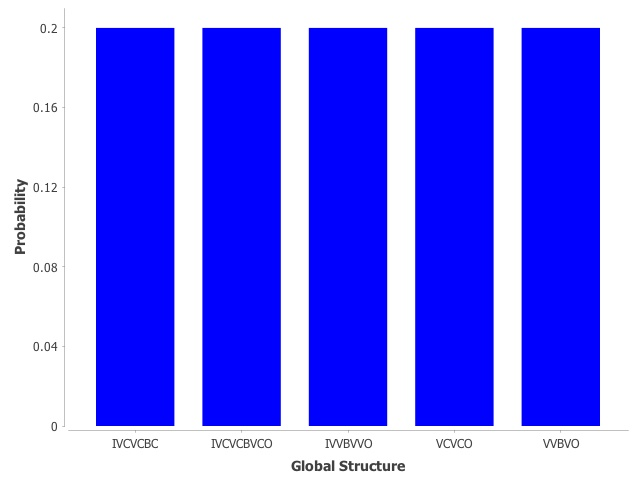
\includegraphics[width=\linewidth]{global_structure}
	\caption{\label{fig:global_structure} A visual representation of a possible probability distribution over global song structures composed of verses (V), choruses (C), intros (I), outros (O), and bridges (B).}
\end{figure}

We improved upon this approximation with a \textbf{distributional model} which learns a multinomial distribution of possible structures from a corpus of composition artefacts (e.g., see Figure~\ref{fig:global_structure}). The disadvantage to the distributional model is that it can only produce structures it has seen before. 

We also implemented a \emph{constrained Markov model}. This model factors $P(\zeta|\nu)$ into a distribution over the number of segments in a song, $P(|\zeta|)$, and a single-order Markov model for sequences of segment types:
\[ P(\zeta|\nu) = P(|\zeta|) P(S_1) \prod_{i=2}^{|\zeta|} P(S_i|S_{i-1}) \]
\noindent An unconstrained, unsmoothed Markov model for $P(S_i|S_{i-1})$ places no guarantee that a sequence of length $|\zeta|$ will be generated, nor that the sequence will end naturally (e.g., with an outro). 

\citeauthor{pachet2001finite}'s constrained Markov model, with which we can constrain the length and the way the sequence ends, modifies the way $P(\zeta|\nu)$ is factored by conditioning $S_i$ on both $i$ and $S_{i-1}$:
\[ P(\zeta|\nu) = P(|\zeta|) P(S_1) \prod_{i=2}^{|\zeta|} P(S_i|i,S_{i-1}) \]
When generating, a length is sampled from $P(|\zeta|)$ and a constrained Markov model for the sampled length is constructed from the unconstrained model with the added constraint that the song must end on an ``end'' token. This model is capable of creating structures of reasonable length and composition that were not seen in the training data. Empirical distributions of $P(|\zeta|)$ and $P(S_i|S_{i-1})$ are shown in Figures~\ref{fig:segment_count_per_song} and~\ref{fig:segment_transitions}.

Another possible solution which we did not try is using a generative grammar, similar to what was done in \cite{steedman1984generative}.

\begin{figure}
	\centering
	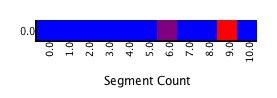
\includegraphics[width=\linewidth]{segment_count_per_song}
	\caption{\label{fig:segment_count_per_song} A visual representation of a possible probability distribution over the number of segments per song. Red corresponds to high probability, blue to low.}
\end{figure}

\begin{figure}[t]
	\centering
	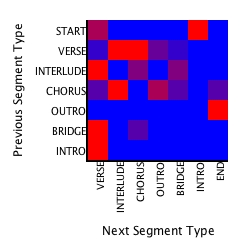
\includegraphics[width=\linewidth]{segment_transitions}
	\caption{\label{fig:segment_transitions} A visual representation of a possible single-order Markov transition matrix for segment types. Red corresponds to high probability, blue to low. The results largely agree with intuition. For example, songs generally start with an intro and occasionally with a verse; songs generally end with an outro and occasionally a chorus; and segments of the same type do not generally follow one another.}
\end{figure}

\subsubsection{Segment Structure, $P(\sigma|\nu,\zeta)$}

In many domains of creativity structure can be thought of hierarchically. For example in a computer game the global structure may describe aspects of the overflow between levels, but the levels themselves also have significant substructural elements that are intuitively independent from the global structure. Though this \emph{segment structure} could be included as part of global structure, modeling this substructure independently leverages principles of abstraction and polymorphism in order to facilitate novel combinations of substructures. For example in story-generation the global structure might dictate something about the abstract content of each paragraph (e.g., protagonist faces a trial, protagonist learns lesson, etc.), whereas the segment structure might define the narrative style for the paragraph (e.g., dramatic visualization, retrospection, dialogue, etc.) or add definition to the abstract content (e.g., the trial is a storm, the trial is losing a loved one, etc.). Modeling these structures independently enables the model to potentially combine narrative styles with plot elements in ways that were not seen during training.

Segments in a composition (e.g., a verse) exhibit segment structure in the number of measures, the number of syllables or notes, which lyrics rhyme or repeat, and patterns in harmony, pitch, or rhythm. We define the distribution over segment structure as
\[ P(\sigma|\nu,\zeta) =  \prod_{i=1}^{|\zeta|} P(C_{\sigma_i} | l_{\sigma_i}) P(l_{\sigma_i}|\zeta_i) \]
\noindent where $\sigma_i$ is the segment structure of $\zeta_i$, $l_{\sigma_i}$ is the length in measures of $\sigma_i$, and $C_{\sigma_i} = ({c_{i1},\mydots,c_{in}})$ is a set of arbitrary size of constraints. 

Constraints define restrictions on different musical viewpoints in order to create rhyme and repetitive motifs. Constraints are defined for a particular viewpoint $v\in\{Harmony, Pitch, Rhythm, Lyric\}$; with a condition $d\in\{Equals, Matches, RhymesWith, HasExpectation\}$; with a boolean value $t$ that defines whether the condition $d$ needs to be satisfied or unsatisfied in order to satisfy the constraint $c_{ij}$; and with $m\in[0,l_{\sigma_i})$ and $b\in[0.0,bpm_m)$ represent the measure and beat offset within the segment to which the constraint applies ($bpm_m$ is the beats per measure of $m$). Each condition $d$ has different sub-variables and dimensionality:

\begin{itemize}
\item $Equals$ conditions - $c_{ij} = \{v,d=Equals,t,m,b,S\}$, where to satisfy $d$, the $v$ token at or near measure $m$, beat $b$ must equal a $v$ token in the set of tokens $S$.
\item $Matches$ conditions - $c_{ij} = \{v,d=Matches,t,m,b,$ $m_2,b_2\}$, where to satisfy $d$ the $v$ tokens at or near measure $m$, beat $b$ and at or near measure $m_2$, beat $b_2$ within the segment must be equal.
\item $RhymesWith$ conditions - $c_{ij} = \{v=Lyric,d=RhymesWith,t,m,b,m_2,b_2\}$, where to satisfy $d$ the $Lyric$ tokens at or near measure $m$, beat $b$ and at or near measure $m_2$, beat $b_2$ within the segment must rhyme.
\item $HasExpectation$ conditions - $c_{ij} = \{v,d=HasExpectation,t,m,b,s\}$, where to satisfy $d$ the $v$ token at or near measure $m$, beat $b$ must have an expectation value above a threshold $s$. This constraint can be used to create a structure of expectation (as discussed in \cite{meyer2008emotion}) in order to model patterns of surprise and tension.
\end{itemize}

Although our system currently only fully implements $RhymesWith$, we include the others to demonstrate there are several potential applications of segment structure.

To approximate $P(\sigma|\zeta)$ we implemented a segment-specific \emph{distributional model} of segment structure which empirically learns $P(l_{\sigma_i}|\zeta_i)$, a probability distribution over segment lengths conditioned on segment type (see Figure~\ref{fig:measure_count_by_segment}) and $P(C_{\sigma_i} | l_{\sigma_i})$, a probability distribution over sets of rhyme scheme constraints conditioned on segment length (see Figure~\ref{fig:segment_structure}).

\begin{figure}
	\centering
	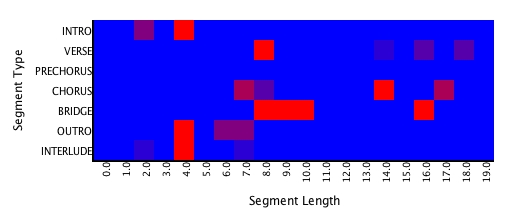
\includegraphics[width=\linewidth]{measure_count_by_segment}
	\caption{\label{fig:measure_count_by_segment} A visual representation of an empirically derived probability distribution over song segment lengths, conditioned on segment type. Red corresponds to high probability, blue to low. The results largely agree with intuition: intros, outros, and interludes tend to be shorter; verses, bridges and choruses tend to be longer.}
\end{figure}

\begin{figure}
	\centering
	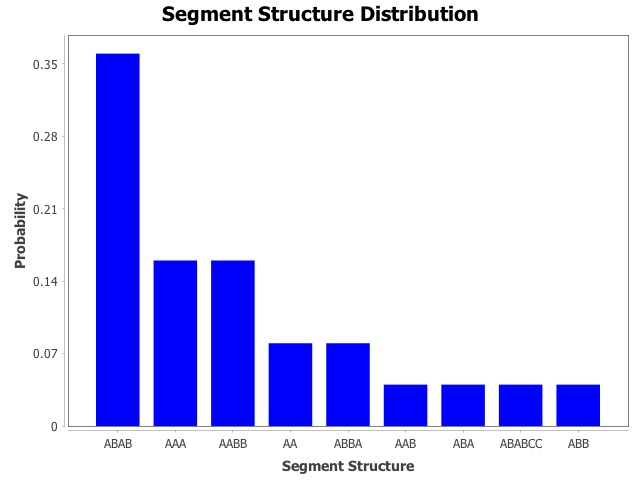
\includegraphics[width=\linewidth]{segment_structure}
	\caption{\label{fig:segment_structure} A visual representation of an empirically derived probability distribution over song segment rhyme structures.}
\end{figure}

Much of the work that has been done with finite-length Markov processes with constraints has required the user to specify the desired constraints in the composition process (e.g., \cite{pachet2014imitative,barbieri2012markov}). This step of learning a model of constraints gives the system increased autonomy to choose its \emph{own} constraints and then generate artefacts to meet those constraints.

With regards to modeling distributions for abstract features of an artifact, empirically-derived distributions can incur significant AI challenges. Training artefacts often fail to label global and even segment structure, and therefore it must be manually labeled or somehow be inferred. Though our current system learns structure from a small manually-annotated subset of the data, our goal in future work is to use sequence alignment over multiple viewpoints to infer global structure, finding regions of an input composition where harmony, melody, and lyrics all match (i.e., chorus) or where only harmony and melody match (i.e., verse). Sequence alignment is also a promising approach to finding segment structure (e.g., \cite{hirjee2010using} use alignment to detect rhyme scheme).

\subsubsection{Harmony, $P(\eta|\nu,\tau)$}

Having modeled an abstract representation of the song, the system proceeds to model the operational representation of the artefact (e.g., paint strokes, narrative text, recipe ingredients, etc.). Whether modeled jointly or factored, the variables describing this concrete representation are conditioned on the constraints imposed by the intention and global/segment structure. Adapting Pachet and Roy's definition of a jazz leadsheet \citeyear{pachet2014imitative}, we define the operational representation of a lyrical composition as parallel sequences of chords $\eta$, notes $\mu$, and lyrics $\lambda$ each with the same total duration. $\eta$, $\mu$, and $\lambda$ are defined in the following sections.

We define a harmony as a sequence of positioned chords $\eta = \{C_1,\mydots,C_n\}$ of arbitrary length. Each position chord $C_i = \{I_i,L_i\}$ has an identity $I_i = \{r_i,q_i,s_i\}$, with root pitch $r_i\in[0,11]$, chord quality $q_i$, and bass pitch $s_i\in[0,11]$; and a position $L_i = \{m_i,b_i\}$, which defines the measure $m_i$ and beat $b_i$ where the chord starts. All models of harmony are normalized to a single key based on the labeled key signature of the training instance at the harmony position.

\begin{figure}[ht]
	\centering
	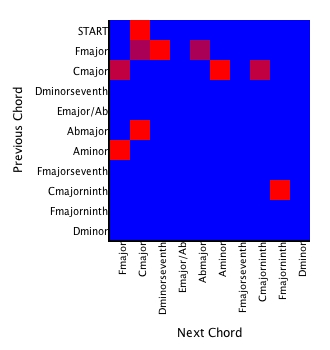
\includegraphics[width=\linewidth]{harmony}
	\caption{\label{fig:harmony} A subsection an empirically derived single-order Markov transition matrix for harmonic chord sequences for chorus segments in 4/4. Red corresponds to high probability, blue to low. As expected for songs normalized to the key of C major, there is high probability that the song starts on a C major chord. }
\end{figure}

In our implementation, we factor $P(\eta|\nu,\tau)$ into independent sequential models regulating chord duration and chord identity:
\[ P(\eta|\nu,\tau) = P(I_1|\tau) P(L_1|\tau) \prod_{i=2} P(I_i|I_{i-1},\tau) P(L_i | L_{i-1},\tau), \]
\noindent the length of the sequence being determined as a function of the duration of the segment to be generated.

The complexity of lyrical composition relative to hand-written characters becomes apparent as we consider several feasible models for approximating both $P(I_i|I_{i-1},\tau)$ and $P(L_i | L_{i-1},\tau)$:

\begin{enumerate}
\item a \textbf{fixed generator} generates a fixed $I$ or $L$, essentially ignoring $\tau$
\item an \textbf{unconditioned Markov model} generates a single sequence for the full length of the composition
\item a \textbf{Markov model} conditioned on $\tau$ in that sequences are generated on a per-segment basis, without conditioning on the segment type
\item \label{model:distribution_model}a \textbf{probability distribution} over tokens conditioned on segment type and the current beat position
\item \label{model:seg_model}a \textbf{Markov model} - one model per segment type
\item a \textbf{hidden Markov model} - hidden states represent the segment type
\end{enumerate}

Of these our implementation uses model~\ref{model:seg_model} for $P(I_i|I_{i-1},\tau)$ (see Figure~\ref{fig:harmony}) and model~\ref{model:distribution_model} for $P(L_i | L_{i-1},\tau)$ (for a discussion of the relative musical merits of each these models see \cite{bodily:inpress-a}). However, it is helpful to recognize that finding the best approximation for a submodel is non-trivial.

The decision to assume that duration and chord are independent, though potentially erroneous, was deliberate. This was based on the reasoning that the strength of a probabilistic model depends on the number of instances used to train the model. Each time a distribution adds a conditional variable, the strength of the model is drastically reduced. We feel that the duration and chord are sufficiently independent to where the model strength recovered by assuming independence outweighed the cost of ignoring any dependence between them.

\subsubsection{Melody, $P(\mu|\nu,\tau,\eta)$}

A melody is a sequence of positioned notes $\mu=\{N_0,\mydots,N_n\}$ of arbitrary length. Each note $N_i = \{p_i,d_i\}$ has a pitch $p_i\in[-1,127]$  (corresponding to a MIDI note value, -1 representing a rest) and a duration $d_i \in \mathbb{R}_{>0}$. We factor $P(\mu|\nu,\tau,\eta)$ into independent sequential models regulating note pitch and duration:
\[ P(\mu|\nu,\tau,\eta) = P(p_1|\eta) P(d_1|\tau) \prod_{i=2} P(p_i|p_{i-1},\eta) P(d_i|d_{i-1},\tau) \]
Of these models only pitch is conditioned on $\eta$. To model $P(p_i|p_{i-1},\eta)$ our implementation uses a single-order Markov chain of scale steps where the scale is defined by the contextual harmony of $\eta$ and to model $P(d_i|d_{i-1},\tau)$ we use a segment-specific Markov chain of note durations.

\begin{figure}[t]
	\centering
	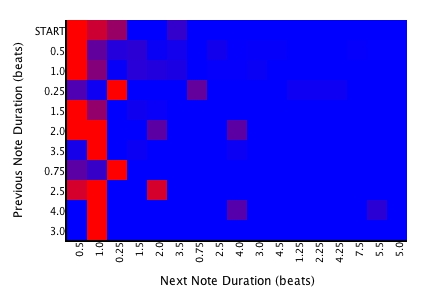
\includegraphics[width=\linewidth]{melody_rhythm}
	\caption{\label{fig:melody_rhythm} A visual representation of an empirically derived single-order Markov model for melodic rhythm durations for verse segments in 4/4. Red corresponds to high probability, blue to low.}
\end{figure}

\subsubsection{Lyrics, $P(\lambda|\nu,\tau,\mu)$}

Several models of natural language generation and in particular NLG in poetry and music have been published \cite{??}. As these models continue to improve, so will their application in lyrical composition. This demonstrates the relative robustness of the HBPL framework: as improved submodels are conceived and implemented, the joint model is also improved.

We define lyrics as a sequence of stressed syllables $\lambda={s_i,\mydots,s_n}$ where $|\lambda| \le |\mu|$. A stressed syllable $s_i = \{t_i, p_i, \epsilon_i\}$ has a text representation $t_i$, a pronunciation (e.g., sequence of ARPAbet phonemes) $p_i$, and a stress $\epsilon_i\in[0,2]$. For each syllable $s_i\in\lambda$ there is a one-to-one relationship with a note $N_i\in\mu$.
\begin{figure*}
	\centering
	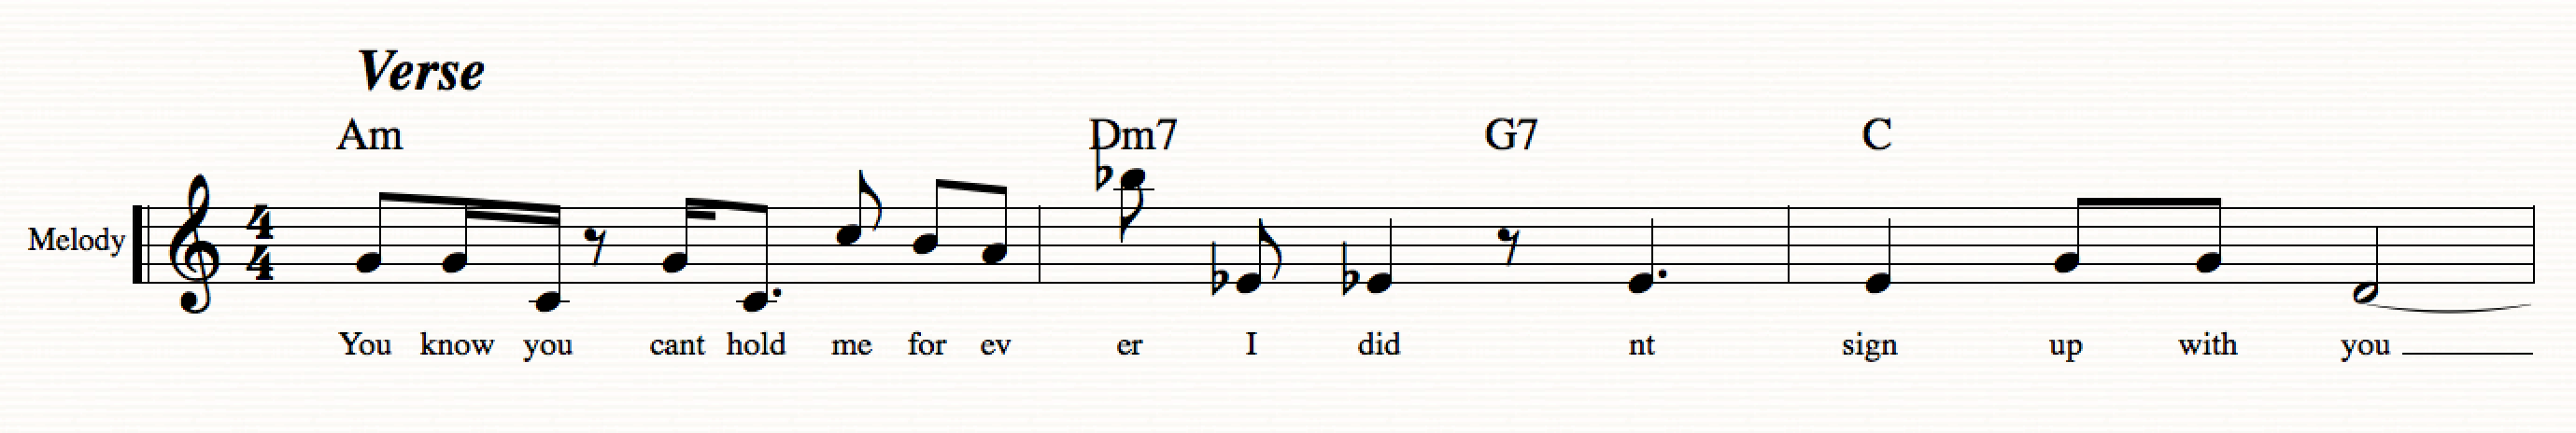
\includegraphics[width=\linewidth]{example}
	\caption{\label{fig:example_composition} The first three measures of a sample composition generated using the HBPL framework. The full composition and others can be seen is available online.}
\end{figure*}

We factor $P(\lambda|\nu,\tau,\mu)$ to construct $\lambda$ as a sequence of lyric phrases $\{\phi_1,\mydots,\phi_n\}$ with the length $l_{phi_i}$ (in syllables) of each phrase computed as a function of the notes in $\mu$ and the rhyme constraints in $\tau$:
\[ P(\lambda|\nu,\tau,\mu) = \prod_{i=1} P(\phi_i | l_{\phi_i}) P(l_{\phi_i} | \mu,\tau) \]
We empirically derived $P(l_{\phi_i} | \mu,\tau)$. For $P(\phi_i | l_{\phi_i})$ we created a probability distribution of lyric templates conditioned on $l_{\phi_i}$ which we used to sample templates. These templates, the $RhymesWith$ constraints of $\tau$, and $\nu$ were given as input to Lyrist \cite{bay:inpress-a}, an independent module we developed for generating novel, intentioned lyrics. Lyrist uses existing lyric segments as syntactic templates for the creation of novel lyric segments. Lyrist intelligently selects words for replacement. Given an original lyric $\lambda$ Lyrist uses the word embedding $W(\lambda)$ to intelligently choose a replacement word $\lambda'$. Lyrist uses the cultural intention of $\nu$ in selecting the training corpus for the word embedding model and the thematic intention of $\nu$ as a seed for finding a set of candidates for $\lambda'$. These candidates are then filtered according to constraints imposed by $\tau$ and the morphosyntactic POS tag of $\lambda$ \cite{bay:inpress-a}.

The advantage of using a template-based approach to lyrics generation is that it does well at maintaining syntactical coherence. The primary shortcomings are that resulting lyrics provide limited syntactic novelty from the training data and make no inherent effort at providing global semantic cohesion.

\subsubsection{A Note on Constrained Markov Models}

\citeauthor{pachet2001finite}'s constrained Markov model requires that the length of the sequence be defined \emph{a priori} \shortcite{pachet2001finite}. One short-coming in our current implementation is that because we have included duration as part of the definition for both harmony and melody (rather than having each chord or note representative of a fixed duration as demonstrated in \cite{pachet2014imitative}) the length of a harmony or melody sequence depends on the durations of each sampled chord or note. While this violates the Markov property and prevents us from being able to effectively use constrained Markov models, we favor the current implementation for reasons related to data sparsity issues and the complexity of implementing higher-order constrained (hidden) Markov model. We hope in the future to overcome both of these hurdles and to shift to ``Markov-friendly'' definitions for melody and harmony in order to incorporate the constraints defined in $tau$ using constrained Markov or constrained hidden Markov models.

\section{Results}

As a proof of concept, we have implemented and trained the described HBPL model on a small corpus of hand-annotated lyrical pop composition data, with all songs normalized to the same starting key. Using this model we generated several compositions (see our website for more examples). Figure~\ref{fig:example_composition} shows an example of a lyrical composition created using the HBPL framework.

\section{Discussion}

The HPBL framework has several important implications which we discuss here.

\subsection{Using the Joint as a Submodel}

Because of its hierarchical nature, a joint model of an artefact class can serve as a submodel for other models. For example, we define the joint probability distribution on inspirations $\iota$, compositions $\gamma$, and voicings $\phi^{(m)}$ as follows,
\[ P(\iota,\gamma,\phi^1, ..., \phi^m) = P(\iota)P(\gamma|\iota) \prod_{m=1}^M P(\phi^m|\iota,\gamma). \]
In essence we are decomposing the model of lyrical song composition to individually model the inspiration for the composition, the symbolic (abstract) representation of the composition, and the concrete rendering of the composition.

\subsubsection{Inspiration, $P(\iota)$}

the method by which intention is defined may be more closely related to an artist or system's ``creative spark''. For example, observers often perceive greater creativity in artefacts which in some way relate to them or to their culture \cite{colton2008creativity}.

Although we did not implement a model of inspiration, it is an area of significant interest for future work. In the joint probability distribution on inspirations $\iota$, compositions $\gamma$, and voicings $\phi^{(m)}$, we define $P(\iota)$ not as the prior on intentions, but as the prior on the inspiring source for the intention. In other words, not ``what was the artefact intended to communicate?'', but ``what was the inspiring source for what the artefact intended to communicate?''

This represents an aspect not present in the model originally presented by \cite{lake2015human}: not only are we modeling \textit{which} artefacts can be generated, but also \textit{why} they are generated. 

In general this demonstrates an unanticipated benefit of factorization: we can condition on any variable that could be argued to influence the composition. Within the long-standing tradition in CC that inspiration is essential to creativity there have been many creative systems in which inspiration is only implicitly defined based on the corpora that the data trains on. With the concept learning framework, we can model this attribute explicitly.

Using an observer's environment or culture as an inspiring source is one possible way to model inspiration. Recent research in Electroencephalogram (EEG)-based affective computing (i.e., reading brain waves) suggests that computers may soon be endowed with perceptive capabilities of an observers emotional state beyond those of their human counterparts \cite{volioti2016mapping}.

\subsubsection{Voicing, $P(\phi^{(m)}|\iota,\gamma)$}

The goal of Pop* was to develop a model of lyrical compositions $\gamma$ (i.e., a leadsheet). However, evaluating such an artefact inevitably requires a concrete rendering of the artefact, whose distribution can we have modeled according to the term $P(\phi^{(m)}|\iota,\gamma)$. We chose a simple voicing module which comps piano chords containing notes defined by the harmony in a middle keyboard range together with a comping bass line (also determined by the harmony). The key for the voiced composition was sampled from the empirical frequency of keys in the training set. 

The artefact is rendered both as leadsheet and a full score (i.e., with piano and bass notes played) in MusicXML format. An MP3 audio featuring computer-sung lyrics recording is then produced using Harmony Assistant (v9.7.0f) and Virtual Singer (v3.2).

\subsubsection{Implications for Recommendation Systems}

In \cite{lake2015human}, the model of $P(\psi)$ given in equation \ref{eq:1} is itself presented as a submodel of the factoring of the joint probability distribution on character types $\psi$, tokens $\omega^m$, and binary images $I^m$:
\[ P(\psi, \theta^1, \mydots,\theta^M,I^1,\mydots,I^M) = P(\psi) \prod_{m=1}^{M} P(I^m|\theta^m)P(\theta^m|\psi), \]
This allows the system to discover motor programs (i.e., abstract character types) from images. By analogy a model for $P(\gamma)$ (similar to the one we just described) could be inserted into a joint probability on composition types $\gamma$, arrangements $\alpha^m$, and audio recordings $\rho^m$,
\[ P(\gamma,\alpha^1,\mydots,\alpha^M,\phi^1,\mydots, \phi^M) = P(\gamma) \prod_{m=1}^M P(\phi^m|\alpha^m)P(\alpha^m|\gamma), \]
\noindent and used to discover abstract composition types from audio recordings (e.g., automatically transcribe sheet music) or to compute probabilities for songs according to different subconcept models of $P(\gamma)$ (e.g., recommendation systems based on harmony, key signature, or melodic pitch or rhythm).

\subsection{Fitness and Self-Evaluation}

The HPBL framework is designed to restrict the generation process \emph{in situ} to producing only meaningful artefacts (as compared to a generate-and-test procedure). As discussed in \cite{ventura2016mere} this ``baked-in'' self-evaluation mechanism has the added benefit of being able to explain to some extent both the novelty, value, and motivation behind generated artefacts. Given its ability to compute probabilities, the HPBL framework could thus also be potentially leveraged as a fitness function for other types of generative models.

\subsection{Big (Need for) Data}

Each of the empirically-driven models requires training on a dataset representative of the artefact domain. Even if we had digital access to all of the compositions ever written, it would represent an infinitesimal portion of the songs that could be written. This is a challenge in many machine learning domains. Unique to the pop music domain, however, is that data is highly proprietary. What \textit{is} available is extremely limited and of relatively poor quality. Compared to natural language, artefacts in music generally require relatively complex representations and relatively few possess the domain knowledge required to generate or transcribe the needed data. Among those who \textit{do} understand and use it, music formatting can vary wildly and inexactly---creating additional challenges for a by-the-bit computer parser. Computers will only learn to speak music as quickly as we either formalize and ubiquitize the language of music \textit{or} endow computers with AI tools (e.g., ears to listen) to fill in the gaps on their own.

The particular challenge of accessing high-quality symbolic \emph{pop} music datasets is significant. There is a dearth of well-annotated resources for those interested in studying any or all of the aspects of pop music composition. There is, however, much we can do to improve the situation. First, we need to make resources that \textit{are} available more accessible (guitar tabs, lyrics sites, beatles). Second, we need to establish a better case for how society and industries stand to benefit from computational pop music research in order to generate a productive dialogue for the support and collaboration of those in possession of large pop music datasets (sheet music sites, spotify, etc., asking for APIs, etc). Note that this is different than asking them to simply give us their proprietary data. Third, we need to recognize contributions of novel datasets.

\section{Conclusion}

The HBPL model is a powerful framework for accomplishing tasks in computational creativity. Using principles of compositionality, causality, and learning-to-learn, the model is able to effectively learn and generate examples of complex creative concepts. Its probabilistic framework lends itself well to modeling important aspects of creativity such as inspiration and intention. The HBPL framework by nature compels researchers in domain-specific subareas of computational creativity to engage in the challenges and debates that the artists themselves are having, namely ``how should an artefact be created?'' and ``does it matter?'' To the extent that these challenges are effectively addressed on the scale of effectively defining and training subconcept models, the HBPL model can be an effective framework for creating and assessing creativity.

\bibliographystyle{iccc}
\bibliography{iccc}

\end{document}
